In this chapter we go into detail about how the DSMC model is implemented in c++. We assume that the reader is familiar with c++ and object orientation. First, we discuss how the code is object oriented and how the different classes are structured. We will explain how particles are divided into collision cells and how the collisions are calculated. The algorithm for detecting and performing surface interactions is discussed, in addition to how the code is parallelized with Message Passing Interface (MPI).


\section{Code structure and variables}
The main function of the program initiates an instance of the class \textit{System} which is the main class of the simulator. It also has an object of the \textit{SystemSampler} class that samples the physical quantities following the definitions in section \ref{sec:dsmc_measuring_physical_quantities}. In this section we go through all of the classes and how they are connected (as shown in figure \ref{fig:dsmc_uml_diagram}). 
\begin{figure}[h]
\begin{center}
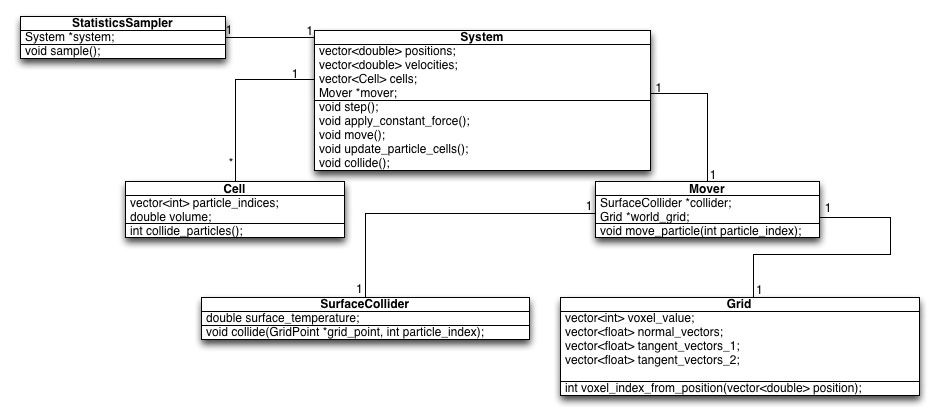
\includegraphics[width=\textwidth, trim=0cm 0cm 0cm 0cm, clip]{DSMC/figures/dsmcuml.png}
\end{center}
\caption{A UML-diagram showing how the classes in the DSMC program are related to each other.}
\label{fig:dsmc_uml_diagram}
\end{figure}
\subsection{main.cpp}
The main function is of course the top level scope of the program. It creates the objects used to read settings, simulate the system and sample statistics. The code is summarized in listing \ref{lst:dsmcmaincpp}.
\begin{lstlisting}[caption=main.cpp, label=lst:dsmcmaincpp]
int main(int args, char* argv[]) {
    // Initialize MPI
    Settings settings("dsmc.ini");
    System system;
    system.initialize(&settings, myid)
    StatisticsSampler sampler(&system);
    
    // Load data from earlier timestep

    for(int timestep=0;timestep<settings.timesteps;timestep++) {
    	system.step();
    	sampler.sample();
    }

    // Save data to file
    // Finalize
}
\end{lstlisting}
\subsection{Class System}
The system class is the top level simulator class. It reads all the physical properties of the system (i.e. system size, density, world geometry) and executes each timestep when it's asked to do so. The phase space variables are saved in 
\begin{itemize}
\item \textit{std::vector<double> r}
\item \textit{std::vector<double> v}
\end{itemize}